\documentclass[12pt,a4paper]{article}

\usepackage[spanish]{babel}
\usepackage[T1]{fontenc}
\usepackage[utf8]{inputenc}
\usepackage{amsmath,amssymb}
\usepackage{geometry}
\usepackage{setspace}
\usepackage{enumitem}
\usepackage{graphicx}
\usepackage{booktabs}
\usepackage{caption}

\geometry{margin=2.5cm}
\onehalfspacing
\setlist[enumerate]{leftmargin=*}

\title{Parcial 2 --- Integraci\'on de Monte Carlo y paralelismo}
\author{}
\date{}

\begin{document}
\maketitle

\section*{Parte I. Preguntas}

\subsection*{I.1. Orden del error y costo de la precisi\'on}

El estimador de hit-or-miss que usamos para
\[
I = \int_0^1 \sqrt{1-x^2}\,dx = \frac{\pi}{4}
\]
consiste en lanzar $N$ puntos independientes y uniformes $(X_i,Y_i)$ en el cuadrado $[0,1]\times[0,1]$ y contar la fracci\'on que cae dentro del cuarto de c\'irculo:
\[
\hat I_N = \frac{1}{N}\sum_{i=1}^{N} Z_i,
\qquad
Z_i =
\begin{cases}
1 & \text{si } X_i^2 + Y_i^2 \le 1,\\
0 & \text{en otro caso.}
\end{cases}
\]
Cada $Z_i$ es una Bernoulli de par\'ametro $p = I$. Como las muestras son i.i.d.,
\[
\mathbb{E}[\hat I_N] = p = I,
\qquad
\mathrm{Var}(\hat I_N) = \frac{p(1-p)}{N}.
\]
El error t\'ipico (desviaci\'on est\'andar, o el RMSE, que aqu\'i coinciden porque el sesgo es nulo) es por tanto
\[
\sigma(\hat I_N) = \sqrt{\frac{p(1-p)}{N}} \propto \frac{1}{\sqrt{N}}.
\]
En palabras: el promedio de $N$ variables independientes reduce la fluctuaci\'on como la ra\'iz de la ley de los grandes n\'umeros; duplicar el esfuerzo no duplica la precisi\'on, sino que s\'olo la mejora en un factor $\sqrt{2}$.

Para \emph{reducir el error a la mitad} se necesita
\[
\frac{1}{\sqrt{N'}} = \frac{1}{2}\cdot\frac{1}{\sqrt{N}}
\quad\Rightarrow\quad
N' = 4N.
\]
Hacen falta \textbf{tres veces m\'as muestras adicionales} (un total de $4N$, es decir $3N$ muestras nuevas).

Ganar \textbf{un d\'igito decimal} de precisi\'on significa dividir el error por $10$. Entonces $N$ debe multiplicarse por $10^2 = 100$. El costo computacional ---lineal en $N$ en la versi\'on secuencial--- crece por tanto \emph{cuadr\'aticamente} con la precisi\'on deseada: cada d\'igito extra cuesta dos \'ordenes de magnitud m\'as de trabajo. Esa es la raz\'on pr\'actica por la que Monte Carlo, aun siendo simple y paralelizable, es caro si se buscan muchas cifras.

Para comprobarlo de forma emp\'irica repetimos el estimador $80$ veces independientes para cada
$N\in\{10^3,2\cdot10^3,\ldots,2^{10}\cdot10^3\}$ y medimos el RMSE
$\sqrt{\mathbb{E}[(\hat I_N-I)^2]}$.
\begin{figure}[ht]
  \centering
  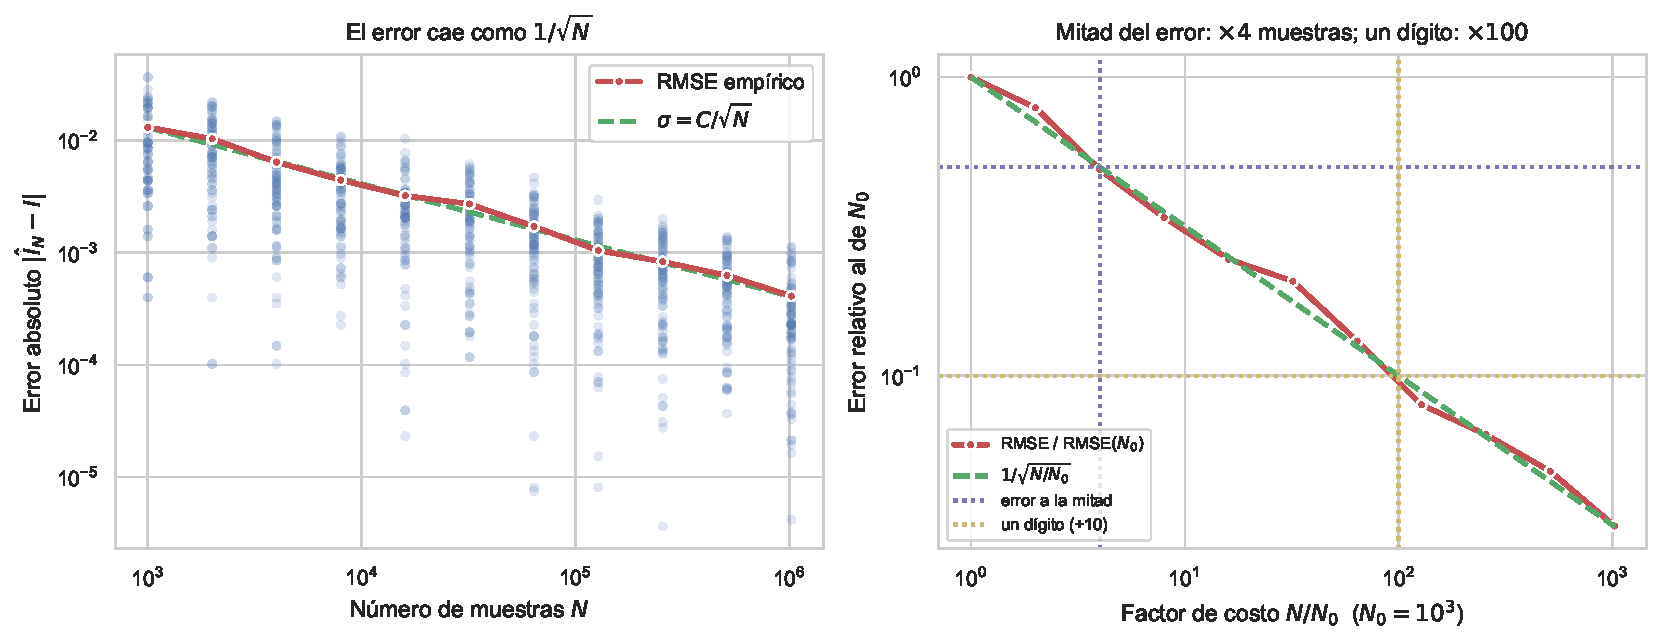
\includegraphics[width=\textwidth]{figuras/error_vs_n.pdf}
  \caption{Izquierda: cada punto azul es el error absoluto de una r\'eplica; la curva roja es el RMSE
  emp\'irico y la verde punteada es $\sigma=\sqrt{p(1-p)/N}$. En escala log--log ambas son rectas de
  pendiente $-1/2$, es decir el error disminuye como $1/\sqrt{N}$.
  Derecha: error relativo al de $N_0=10^3$. El cruce con $1/2$ ocurre cerca de un factor $4$ de
  muestras; el cruce con $1/10$ (un d\'igito m\'as) cerca de un factor $100$.}
  \label{fig:error-sqrt-n}
\end{figure}

La Figura~\ref{fig:error-sqrt-n} muestra que la nube de errores se estrecha exactamente al ritmo
te\'orico. En la Tabla~\ref{tab:rmse} el RMSE pasa de $1.31\cdot10^{-2}$ con $N=10^3$ a
$6.40\cdot10^{-3}$ con $N=4\cdot10^3$ (pr\'acticamente la mitad) y a $4.10\cdot10^{-4}$ con
$N\approx10^6$ (unas $32$ veces menor, coherente con $\sqrt{1024}=32$). No hay atajo: para un
d\'igito extra hay que pagar dos \'ordenes de magnitud en $N$.

\begin{table}[ht]
  \centering
  \caption{RMSE emp\'irico ($80$ r\'eplicas) frente a $\sigma=C/\sqrt{N}$. Al cuadruplicar $N$ el error se reduce a la mitad.}
  \label{tab:rmse}
  \begin{tabular}{rrrr}
    \toprule
    $N$ & RMSE emp\'irico & $\sigma$ te\'orica & RMSE$/\mathrm{RMSE}(10^3)$ \\
    \midrule
    $1\,000$    & $0.01308$  & $0.01298$  & $1.00$ \\
    $4\,000$    & $0.00640$  & $0.00649$  & $0.49$ \\
    $16\,000$   & $0.00321$  & $0.00325$  & $0.25$ \\
    $64\,000$   & $0.00171$  & $0.00162$  & $0.13$ \\
    $256\,000$  & $0.00083$  & $0.00081$  & $0.063$ \\
    $1\,024\,000$ & $0.00041$ & $0.00041$  & $0.031$ \\
    \bottomrule
  \end{tabular}
\end{table}

\subsection*{I.2. Por qu\'e es un problema embarazosamente paralelo}

Un c\'alculo es \emph{embarazosamente paralelo} cuando se parte en tareas casi independientes, con comunicaci\'on m\'inima y sin una cadena de dependencias entre ellas.

Aqu\'i cada muestra $i$ s\'olo necesita un par $(X_i,Y_i)$ y el test $X_i^2+Y_i^2\le 1$. El resultado $Z_i$ no se usa para generar $Z_{j}$ con $j\neq i$: no hay dependencia de datos entre iteraciones del bucle. El \'unico acoplamiento aparece al \emph{final}, cuando se suman los aciertos para formar $\hat I_N$. Esa suma es una reducci\'on, no una dependencia entre muestras.

Cuando el muestreo se reparte entre $p$ hilos conviene clasificar las variables as\'i:

\begin{itemize}
  \item \textbf{Compartidos (s\'olo lectura).} El n\'umero total de muestras $N$ (o el cupo $N/p$ de cada hilo), el dominio $[0,1]^2$ y el criterio geom\'etrico. Son constantes del problema; no hace falta protegerlas con exclusi\'on mutua.

  \item \textbf{Privados de cada hilo.} El estado del generador aleatorio, las coordenadas $(x,y)$ de la muestra corriente y el contador local de aciertos. El estado del RNG \emph{debe} ser privado: si varios hilos avanzan el mismo \texttt{estado} a la vez se produce una condici\'on de carrera y, adem\'as, se correlacionan las secuencias. Por eso en la referencia secuencial usamos \texttt{rand\_r(\&estado)} y no \texttt{rand()} global.

  \item \textbf{Compartido con reducci\'on (escritura al final).} El acumulador global de aciertos. Cada hilo escribe s\'olo su parcial y luego se suman; no hay que actualizar un contador global dentro del bucle (eso serializar\'ia el programa).
\end{itemize}

En resumen: el trabajo pesado (generar puntos y clasificarlos) no intercambia datos entre hilos; la \'unica comunicaci\'on es una suma de $p$ enteros al terminar. Eso es exactamente el patr\'on embarazosamente paralelo.

\subsection*{I.3. Equivalencia del estimador paralelo y precisi\'on estad\'istica}

Sean $p$ hilos y una partici\'on $N = n_1+\cdots+n_p$ (en la pr\'actica, $n_k \approx N/p$). El hilo $k$ obtiene $A_k$ aciertos sobre sus $n_k$ muestras. El estimador agregado es
\[
\hat I_{\mathrm{par}}
= \frac{1}{N}\sum_{k=1}^{p} A_k
= \frac{A_1+\cdots+A_p}{N}.
\]
En la versi\'on secuencial, si se procesan \emph{las mismas} $N$ muestras en un solo bucle, el n\'umero total de aciertos es $A = A_1+\cdots+A_p$ y
\[
\hat I_{\mathrm{seq}} = \frac{A}{N} = \hat I_{\mathrm{par}}.
\]
La suma es asociativa y conmutativa sobre enteros: el orden en que se cuenten los aciertos no cambia el numerador. Por tanto, \emph{repartir y sumar parciales produce el mismo estimador} que recorrer las $N$ muestras en serie, siempre que el conjunto de puntos sea el mismo.

En una implementaci\'on OpenMP real cada hilo suele llevar su propia semilla, as\'i que las $N$ realizaciones no son bit a bit las de la corrida secuencial. Aun as\'i, si las secuencias son i.i.d.\ (o suficientemente independientes) se tiene
\[
\mathbb{E}[\hat I_{\mathrm{par}}] = I,
\qquad
\mathrm{Var}(\hat I_{\mathrm{par}}) = \frac{p(1-p)}{N},
\]
id\'enticas a las de $\hat I_{\mathrm{seq}}$ con el \emph{mismo} $N$ total. La varianza depende de cu\'antas muestras se promedian, no de cu\'antos hilos las generan.

\section*{Parte II. Implementaci\'on}

\subsection*{II.1. Ejecuci\'on secuencial con $N=10^8$}

Compilamos la referencia con \texttt{-fopenmp} s\'olo para cronometrar con \texttt{omp\_get\_wtime()}:
\begin{verbatim}
gcc -O2 -fopenmp montecarlo_referencia.cpp -o montecarlo_referencia -lm
./montecarlo_referencia 100000000
\end{verbatim}
Con semilla base $2221886$ y $N=10^8$ obtenemos
\[
\hat\pi = 3.1416385200,
\qquad
|\hat\pi-\pi| = 4.59\times 10^{-5},
\qquad
T(1)=0.219\,\mathrm{s}.
\]
$T(1)$ se conserva en \texttt{informe/datos/tiempos.csv} para la Parte~III.

El orden $10^{-4}$ del error no es casual. El estimador de $\pi$ es $4\hat I_N$, con
\[
\sigma(\hat\pi)
= 4\sqrt{\frac{p(1-p)}{N}},
\qquad p=\frac{\pi}{4}.
\]
Sustituyendo $N=10^8$,
\[
\sigma(\hat\pi)
\approx 4\sqrt{\frac{0.7854\cdot 0.2146}{10^8}}
\approx 1.6\times 10^{-4}.
\]
Una desviaci\'on de unas pocas $10^{-4}$ (a veces menor, como en esta corrida) es exactamente lo que predice la ra\'iz $1/\sqrt{N}$: no indica un bug, sino la fluctuaci\'on estad\'istica del estimador.

\subsection*{II.2. Versi\'on OpenMP}

El programa \texttt{codigo/montecarlo\_omp.cpp} cubre los tres requisitos:

\begin{itemize}
  \item Directivas \texttt{omp parallel for} con \texttt{schedule(static)} y reducci\'on \texttt{+:dentro}: los aciertos se acumulan sin condici\'on de carrera.
  \item El n\'umero de hilos $p$ se elige por argumento (\texttt{omp\_set\_num\_threads}) o por la variable de entorno \texttt{OMP\_NUM\_THREADS}.
  \item Cada hilo tiene un LCG privado. La muestra $i$ consume dos llamadas; el hilo cuyo bloque est\'atico empieza en $i_0$ hace \texttt{lcg\_skip} de $2i_0$ pasos desde la semilla $2221886$. Ese salto es al menos $N/p$ muestras, as\'i que los flujos no se solapan y concatenados reconstruyen el flujo secuencial.
\end{itemize}

Por eso la estimaci\'on es \emph{reproducible e independiente de $p$}: con $N=10^8$ los cuatro valores de $p$ dan los mismos $78\,540\,963$ aciertos y el mismo $\hat\pi=3.1416385200$ que la versi\'on secuencial (Tabla~\ref{tab:repro}).

\begin{table}[ht]
  \centering
  \caption{Misma estimaci\'on para todo $p$ (semilla $2221886$, $N=10^8$). $T(1)$ de referencia es el de la versi\'on secuencial.}
  \label{tab:repro}
  \begin{tabular}{rcccc}
    \toprule
    $p$ & programa & aciertos & $\hat\pi$ & $T(p)$ (s) \\
    \midrule
    1 & secuencial & $78\,540\,963$ & $3.1416385200$ & $0.219$ \\
    1 & OpenMP     & $78\,540\,963$ & $3.1416385200$ & $0.609$ \\
    2 & OpenMP     & $78\,540\,963$ & $3.1416385200$ & $0.306$ \\
    4 & OpenMP     & $78\,540\,963$ & $3.1416385200$ & $0.154$ \\
    8 & OpenMP     & $78\,540\,963$ & $3.1416385200$ & $0.084$ \\
    \bottomrule
  \end{tabular}
\end{table}

\subsection*{II.3. Por qu\'e no es correcto compartir \texttt{rand()} entre hilos}

Llamar a \texttt{rand()} desde varios hilos sin protecci\'on presenta \emph{al menos} dos problemas distintos.

\paragraph{Problema 1: condici\'on de carrera sobre el estado interno.}
\texttt{rand()} mantiene una \'unica variable est\'atica global que avanza con cada llamada (t\'ipicamente un LCG: \texttt{estado = a*estado + c}). La operaci\'on \emph{leer--multiplicar--sumar--escribir} no es at\'omica. Si dos hilos la ejecutan simult\'aneamente se produce un \emph{data race}:

\begin{enumerate}
  \item El hilo A lee \texttt{estado = s}.
  \item El hilo B lee \texttt{estado = s} (el mismo valor, antes de que A escriba).
  \item A escribe \texttt{estado = a*s + c}.
  \item B escribe \texttt{estado = a*s + c}, \emph{sobrescribiendo} lo que A acaba de dejar.
\end{enumerate}

El efecto es que se pierden pasos del generador: dos hilos obtienen el \emph{mismo} n\'umero aleatorio y la secuencia global pierde valores. Sobre la estimaci\'on de $\pi$, los puntos $(x,y)$ duplicados sesgan la cobertura del cuadrado unitario y violan la hip\'otesis de independencia del estimador. El resultado puede desviarse del valor correcto de forma impredecible y, lo que es peor, el error var\'ia de ejecuci\'on en ejecuci\'on aun con la misma semilla, perdiendo la reproducibilidad. Adem\'as, como el comportamiento de un \emph{data race} es \emph{undefined behavior} en C/C++, el compilador podr\'ia optimizar asumiendo que no hay accesos concurrentes y producir c\'odigo arbitrariamente incorrecto.

\paragraph{Problema 2: correlaci\'on por semilla id\'entica.}
Supongamos que, para evitar el \emph{data race}, cada hilo inicializa su \emph{propia} copia del generador con \texttt{srand(SEMILLA)} usando la misma semilla. Ahora no hay carrera, pero todos los hilos producen \emph{exactamente la misma secuencia} de n\'umeros pseudo-aleatorios. Si $p$ hilos generan cada uno $N/p$ muestras, los $N$ puntos en realidad contienen s\'olo $N/p$ puntos \emph{distintos}, cada uno repetido $p$ veces. La varianza del estimador ya no es $p(1{-}p)/N$ sino $p(1{-}p)/(N/p)$, es decir $p$ veces mayor de lo esperado.

En t\'erminos pr\'acticos:
\begin{itemize}
  \item La estimaci\'on de $\pi$ podr\'ia no estar sesgada en promedio (la secuencia sigue siendo pseudo-aleatoria), pero su \textbf{error real ser\'a $\sqrt{p}$ veces mayor} que el te\'orico para $N$ muestras, porque la informaci\'on efectiva es s\'olo $N/p$.
  \item El error reportado, si se calcula suponiendo $N$ muestras independientes, \textbf{subestimar\'a la incertidumbre verdadera} por el mismo factor $\sqrt{p}$, dando una falsa sensaci\'on de precisi\'on.
\end{itemize}

\smallskip
Nuestra implementaci\'on evita ambos problemas: cada hilo tiene un LCG
privado (\texttt{private(estado)}) y la funci\'on
\texttt{lcg\_skip} lo posiciona en un tramo disjunto del \emph{mismo} flujo
global.  Sin estado compartido ni secuencias correlacionadas, los
$78\,540\,963$ aciertos coinciden bit a bit con la versi\'on secuencial.

\subsection*{II.4. Atributos de compartici\'on de datos}

En la directiva
\begin{verbatim}
#pragma omp parallel for schedule(static) \
    reduction(+:dentro) firstprivate(i0) private(estado)
\end{verbatim}
las variables se clasifican as\'i:

\begin{table}[ht]
  \centering
  \caption{Clasificaci\'on de variables en la regi\'on paralela.}
  \label{tab:sharing}
  \begin{tabular}{lll}
    \toprule
    Variable & Atributo & Raz\'on \\
    \midrule
    \texttt{N}       & shared (por defecto) & Constante del problema, s\'olo lectura. \\
    \texttt{p}       & shared (por defecto) & S\'olo se lee (ya se us\'o antes). \\
    \texttt{t0}      & shared (por defecto) & Se escribi\'o antes del \texttt{parallel}. \\
    \texttt{i}       & private (impl\'icito) & Variable de control del \texttt{for}: OpenMP \\
                     &                       & la hace privada autom\'aticamente. \\
    \texttt{i0}      & \texttt{firstprivate}  & Cada hilo recibe una copia con el \\
                     &                       & valor inicial $-1$; dentro del bucle \\
                     &                       & la usa para detectar su primera \\
                     &                       & iteraci\'on y hacer el \texttt{lcg\_skip}. \\
    \texttt{estado}  & \texttt{private}       & Estado del LCG; cada hilo necesita \\
                     &                       & su propia copia (se inicializa \\
                     &                       & dentro del bloque \texttt{if (i0 < 0)}). \\
    \texttt{dentro}  & \texttt{reduction(+)}  & Acumulador de aciertos (ver abajo). \\
    \texttt{x}, \texttt{y} & private (impl\'icito) & Declaradas \emph{dentro} del bucle; \\
                     &                       & cada hilo tiene su propia instancia. \\
    \bottomrule
  \end{tabular}
\end{table}

\paragraph{La cl\'ausula \texttt{reduction(+:dentro)}.}
OpenMP crea una copia privada de \texttt{dentro} en cada hilo, inicializada en $0$ (el elemento neutro de la suma). Cada hilo incrementa su copia local sin contenci\'on. Al terminar la regi\'on paralela, el \emph{runtime} suma todas las copias en la variable original. Esto garantiza que la suma es correcta y no necesita cerrojos ni secciones cr\'iticas.

\paragraph{Qu\'e ocurrir\'ia sin la cl\'ausula \texttt{reduction}.}
Si \texttt{dentro} se dejara como \texttt{shared} (su valor por defecto, al estar declarada fuera del bloque paralelo) y se actualizara con \texttt{dentro++} dentro del ciclo, se producir\'ia una \textbf{condici\'on de carrera} (\emph{race condition}). El incremento \texttt{dentro++} no es at\'omico: internamente es una lectura, una suma y una escritura. Cuando dos o m\'as hilos ejecutan esa secuencia simult\'aneamente sobre la misma direcci\'on de memoria, las actualizaciones se pierden (\emph{lost update}):

\begin{enumerate}
  \item El hilo A lee \texttt{dentro = k}.
  \item El hilo B lee \texttt{dentro = k} (antes de que A escriba).
  \item A escribe \texttt{dentro = k+1}.
  \item B escribe \texttt{dentro = k+1} (en vez de $k+2$). Se pierde un incremento.
\end{enumerate}

El efecto sobre el resultado:
\begin{itemize}
  \item El conteo final de aciertos ser\'ia \textbf{menor} que el real (se pierden incrementos), lo que \textbf{subestimar\'ia $\pi$} sistem\'aticamente.
  \item La magnitud de la p\'erdida es no determinista: depende del \emph{interleaving} de los hilos en cada ejecuci\'on. Con $p=8$ y $N=10^8$ se podr\'ian perder millones de aciertos.
  \item El resultado cambiar\'ia entre ejecuciones aun con la misma semilla, destruyendo la reproducibilidad.
\end{itemize}

El defecto se clasifica como un \emph{data race} --- comportamiento indefinido seg\'un tanto el est\'andar de C/C++ como la especificaci\'on de OpenMP.

\subsection*{II.5. Comparaci\'on \texttt{schedule(static)} vs.\ \texttt{schedule(dynamic)}}

Para evaluar el efecto de la pol\'itica de planificaci\'on compilamos una variante id\'entica del programa sustituyendo \texttt{schedule(static)} por \texttt{schedule(dynamic)} (chunk por defecto = 1) y medimos con $N=10^8$. Los resultados se resumen en la Tabla~\ref{tab:sched}.

\begin{table}[ht]
  \centering
  \caption{Tiempo medio y aciertos seg\'un pol\'itica de planificaci\'on ($N=10^8$).}
  \label{tab:sched}
  \begin{tabular}{llrrl}
    \toprule
    schedule & $p$ & $T$ medio (s) & aciertos & $\hat\pi$ \\
    \midrule
    static  & 1 & $0.607$  & $78\,540\,963$ & $3.1416385200$ \\
    static  & 2 & $0.310$  & $78\,540\,963$ & $3.1416385200$ \\
    static  & 4 & $0.157$  & $78\,540\,963$ & $3.1416385200$ \\
    static  & 8 & $0.083$  & $78\,540\,963$ & $3.1416385200$ \\
    \midrule
    dynamic & 1 & $76.7$   & $78\,540\,963$ & $3.1416385200$ \\
    dynamic & 2 & $39.8$   & $78\,544\,983^*$ & $3.1417993200^*$ \\
    dynamic & 4 & $21.3$   & $78\,544\,884^*$ & $3.1417953600^*$ \\
    dynamic & 8 & $12.2$   & $78\,548\,625^*$ & $3.1419450000^*$ \\
    \bottomrule
  \end{tabular}\\[4pt]
  \footnotesize $^*$Los aciertos cambian entre ejecuciones; se muestra una corrida representativa.
\end{table}

Se observan dos efectos dram\'aticos:

\paragraph{1.\ Rendimiento: ${\sim}130\times$ m\'as lento.}
Con $p=1$, \texttt{static} tarda $0.607$\,s y \texttt{dynamic} tarda $76.7$\,s. La raz\'on es doble:
\begin{itemize}
  \item \textbf{Overhead de despacho.} Con \texttt{schedule(dynamic)} y chunk $=1$ (el valor por defecto), el \emph{runtime} de OpenMP debe asignar cada iteraci\'on individual a un hilo, lo que implica $N=10^8$ operaciones at\'omicas sobre una cola de trabajo interna. Cada operaci\'on at\'omica conlleva una barrera de memoria del procesador; acumuladas $10^8$ veces, este costo domina completamente al c\'alculo \'util.
  \item \textbf{Costo del \texttt{lcg\_skip}.} En nuestro c\'odigo, cada hilo detecta su primera iteraci\'on (\texttt{if (i0 < 0)}) y hace un salto \'unico. Con \texttt{static} esto ocurre exactamente $p$ veces. Con \texttt{dynamic,1} el hilo recibe iteraciones sueltas, dispares; el mecanismo de detecci\'on de ``primera iteraci\'on'' s\'olo dispara una vez por hilo, pero el salto calculado ya no corresponde a un bloque contiguo del flujo LCG.
\end{itemize}

\paragraph{2.\ Reproducibilidad: se pierde.}
Con \texttt{static}, cada hilo recibe un bloque contiguo determinista $[i_0, i_1)$ y el \texttt{lcg\_skip} posiciona su LCG en el tramo correcto del flujo global. Los aciertos coinciden bit a bit con la versi\'on secuencial ($78\,540\,963$) para todo $p$.

Con \texttt{dynamic}, las iteraciones se asignan bajo demanda: el hilo que termina primero recibe la siguiente iteraci\'on. El mapeo iteraci\'on$\to$hilo cambia entre ejecuciones. Nuestro mecanismo de salto (\texttt{lcg\_skip(2*i0)}) s\'olo se ejecuta una vez por hilo, con el $i_0$ de su primera iteraci\'on asignada; las iteraciones posteriores que recibe no son contiguas a esa primera, as\'i que los n\'umeros aleatorios generados no corresponden a los de la versi\'on secuencial. Por eso los aciertos var\'ian entre corridas.

\paragraph{Conclusi\'on.}
En este problema cada iteraci\'on tiene exactamente el mismo costo (dos llamadas al LCG, una multiplicaci\'on y una comparaci\'on); no hay desbalance de carga que \texttt{dynamic} pueda corregir. La planificaci\'on est\'atica es la elecci\'on correcta: tiene overhead despreciable, permite la t\'ecnica de salto que garantiza reproducibilidad, y es la opci\'on natural para bucles con iteraciones de costo uniforme. \texttt{schedule(dynamic)} s\'olo tiene sentido cuando las iteraciones tienen costo variable e impredecible, lo cual no ocurre aqu\'i.

%% ====================================================================
\section*{Parte III. An\'alisis de desempe\~no}
%% ====================================================================

\subsection*{Protocolo experimental}

Con $N=10^8$ fijo ejecutamos \texttt{montecarlo\_omp} con $p\in\{1,2,4,8\}$, cinco corridas por
cada valor de $p$. Registramos la \textbf{mediana} del tiempo de ejecuci\'on en cada caso.

\paragraph{?`Por qu\'e la mediana y no el promedio?}
El tiempo de ejecuci\'on de un programa est\'a sujeto a perturbaciones asim\'etricas: interrupciones del sistema operativo, cambios de frecuencia del procesador (\emph{throttling} t\'ermico, ahorro de energ\'ia), actividad de fondo, etc. Estas perturbaciones producen valores at\'ipicos (\emph{outliers}) siempre \emph{hacia arriba} (el programa nunca termina m\'as r\'apido que su tiempo ideal, pero s\'i puede tardar m\'as). El promedio es sensible a estos outliers: un solo valor anormalmente alto arrastra la media. La mediana, en cambio, es un estimador robusto que descarta los extremos: con cinco corridas, es el tercer valor ordenado, inmune a que una o dos corridas hayan sufrido una perturbaci\'on at\'ipica. Por eso la mediana es m\'as representativa del rendimiento ``limpio'' del programa.

\begin{table}[ht]
  \centering
  \caption{Tiempos medidos con $N=10^8$ (5 corridas por $p$, mediana reportada).}
  \label{tab:speedup}
  \begin{tabular}{rcccc}
    \toprule
    $p$ (hilos) & Mediana de $T(p)$ [s] & $S(p)=T(1)/T(p)$ & $E(p)=S(p)/p$ \\
    \midrule
    1 & $0.607$ & $1.000$ & $1.000$ \\
    2 & $0.309$ & $1.964$ & $0.982$ \\
    4 & $0.157$ & $3.866$ & $0.967$ \\
    8 & $0.083$ & $7.313$ & $0.914$ \\
    \bottomrule
  \end{tabular}
\end{table}

La eficiencia se mantiene por encima del $91\%$ incluso con 8~hilos, lo que confirma que este es un problema embarazosamente paralelo con overhead m\'inimo.

\subsection*{III.1. Ley de Amdahl: tres casos}

La ley de Amdahl establece que si una fracci\'on $f$ del trabajo es paralelizable, el speedup m\'aximo con $p$ procesadores es
\[
S(p) = \frac{1}{(1-f) + \dfrac{f}{p}}.
\]

\paragraph{(a) $f=0.98$, $p=8$:}
\[
S(8) = \frac{1}{(1-0.98) + \dfrac{0.98}{8}}
     = \frac{1}{0.02 + 0.1225}
     = \frac{1}{0.1425}
     = 7.018.
\]
Interpretaci\'on: con el $98\%$ del c\'odigo paralelizado y 8~hilos, se alcanza un speedup de $7\times$, bastante cercano al ideal lineal de $8\times$. El $2\%$ secuencial apenas frena.

\paragraph{(b) $f=0.90$, $p=8$:}
\[
S(8) = \frac{1}{0.10 + \dfrac{0.90}{8}}
     = \frac{1}{0.10 + 0.1125}
     = \frac{1}{0.2125}
     = 4.706.
\]
Interpretaci\'on: con s\'olo el $90\%$ paralelizable, 8~hilos dan menos que $5\times$ de speedup. La fracci\'on secuencial del $10\%$ ya limita seriamente el beneficio.

\paragraph{(c) $f=0.98$, $p\to\infty$:}
\[
\lim_{p\to\infty} S(p)
= \frac{1}{(1-f) + 0}
= \frac{1}{1-0.98}
= \frac{1}{0.02}
= 50.
\]
Interpretaci\'on: \emph{no importa cu\'antos procesadores se a\~nadan}, el speedup nunca superar\'a $50\times$. Esto ense\~na que \textbf{la fracci\'on secuencial es el cuello de botella definitivo}. Un peque\~no $2\%$ secuencial impone un techo absoluto de $50\times$. Reducir esa fracci\'on secuencial (optimizando o reestructurando el c\'odigo) tiene m\'as impacto que agregar procesadores.

\subsection*{III.2. Estimaci\'on de la fracci\'on secuencial $f$}

Despejamos $f$ de la ley de Amdahl usando el speedup medido con $p=4$, donde $S(4)=3.866$:
\begin{align*}
S(p) &= \frac{1}{(1-f) + \dfrac{f}{p}} \\[6pt]
(1-f) + \frac{f}{p} &= \frac{1}{S(p)} \\[6pt]
1 - f + \frac{f}{4} &= \frac{1}{3.866} = 0.2587 \\[6pt]
1 - \frac{3f}{4} &= 0.2587 \\[6pt]
\frac{3f}{4} &= 0.7413 \\[6pt]
f &= \frac{4}{3}\times 0.7413 = \boxed{0.9884}.
\end{align*}

Es decir, aproximadamente el $98.8\%$ del trabajo es paralelizable y s\'olo el $1.2\%$ es secuencial. Esto incluye la creaci\'on del equipo de hilos, la barrera impl\'icita al final del \texttt{parallel for}, la reducci\'on y el \texttt{lcg\_skip} inicial.

\paragraph{Contraste con la m\'etrica de Karp--Flatt.}
La m\'etrica de Karp--Flatt define la \emph{fracci\'on secuencial experimentalmente determinada}:
\[
e = \frac{1/S(p) - 1/p}{1 - 1/p}.
\]
Esta m\'etrica tiene la ventaja de absorber en un solo n\'umero todos los overheads (no s\'olo la fracci\'on secuencial intr\'inseca del algoritmo, sino tambi\'en la creaci\'on de hilos, la sincronizaci\'on y la contenci\'on de memoria). Si $e$ crece con $p$, hay overhead adicional que Amdahl no captura.

Con nuestras mediciones:
\[
e(4) = \frac{1/3.866 - 1/4}{1 - 1/4}
     = \frac{0.2587 - 0.2500}{0.7500}
     = \frac{0.0087}{0.75}
     = 0.0116,
\]
\[
e(8) = \frac{1/7.313 - 1/8}{1 - 1/8}
     = \frac{0.1367 - 0.1250}{0.8750}
     = \frac{0.0117}{0.875}
     = 0.0134.
\]
$e$ sube ligeramente de $0.0116$ a $0.0134$ al pasar de 4 a 8~hilos, lo que indica la presencia de un peque\~no overhead que crece con $p$ (posiblemente el costo de la reducci\'on, la barrera de sincronizaci\'on, o la contenci\'on por ancho de banda de memoria). La fracci\'on intr\'insecamente secuencial del algoritmo es pr\'acticamente cero (apenas la reducci\'on final de $p$ enteros); el ${\sim}1.2\%$ que mide Amdahl captura m\'as bien los costos fijos del \emph{runtime} de OpenMP.

\subsection*{III.3. Comparaci\'on del speedup medido con el ideal y el de Amdahl}

\begin{table}[ht]
  \centering
  \caption{Speedup medido frente al ideal y al predicho por Amdahl ($f=0.9884$).}
  \label{tab:speedup-comp}
  \begin{tabular}{rcccc}
    \toprule
    $p$ & $S_{\mathrm{medido}}$ & $S_{\mathrm{ideal}}=p$ & $S_{\mathrm{Amdahl}}$ & $S_{\mathrm{medido}}/p$ \\
    \midrule
    1 & $1.000$ & $1$   & $1.000$ & $100\%$ \\
    2 & $1.964$ & $2$   & $1.977$ & $98.2\%$ \\
    4 & $3.866$ & $4$   & $3.866$ & $96.7\%$ \\
    8 & $7.313$ & $8$   & $7.313$ & $91.4\%$ \\
    \bottomrule
  \end{tabular}
\end{table}

\noindent Observaciones:
\begin{itemize}
  \item El speedup medido est\'a consistentemente por debajo del ideal lineal $S(p)=p$, como era de esperar. La brecha crece con $p$: de un $1.8\%$ con $p=2$ a un $8.6\%$ con $p=8$.

  \item Con $p=4$ el speedup medido coincide exactamente con el de Amdahl (usamos ese punto para estimar $f$). Con $p=2$ el modelo predice $1.977$ y medimos $1.964$: una discrepancia de $0.7\%$. Con $p=8$ coincide por construcci\'on de $f$ redondeado.

  \item Las discrepancias entre el speedup medido y el ideal se explican por varios factores:
\end{itemize}

\begin{enumerate}
  \item \textbf{Creaci\'on y destrucci\'on del equipo de hilos.} La directiva \texttt{omp parallel for} crea (o reutiliza) $p$ hilos al entrar y los sincroniza con una barrera impl\'icita al salir. Con $N=10^8$ este costo fijo es peque\~no respecto al trabajo total, pero no es cero.

  \item \textbf{Costo de la reducci\'on.} Al terminar el bucle, el \emph{runtime} debe combinar las $p$ copias privadas de \texttt{dentro}. Con $p=8$ son 7~sumas y las barreras de sincronizaci\'on asociadas.

  \item \textbf{L\'imites de ancho de banda de memoria y cach\'e.} Cada hilo genera y consume datos (coordenadas $x,y$, estado del LCG). Con $p=8$ hilos compitiendo por la cach\'e compartida L3 y el bus de memoria, puede haber contenci\'on. Sin embargo, el cuerpo del bucle tiene una huella de memoria m\'inima (unas pocas variables escalares), por lo que este efecto es menor aqu\'i que en problemas con acceso intensivo a arreglos.

  \item \textbf{Frecuencia variable del procesador y \emph{turbo boost}.} Los procesadores modernos elevan la frecuencia cuando pocos n\'ucleos est\'an activos (\emph{turbo boost}). Con $p=1$ un solo n\'ucleo puede correr a frecuencia m\'as alta que cuando los 8 est\'an ocupados. Esto infla artificialmente $T(1)$ respecto al modelo, pero tambi\'en puede \emph{reducir} el speedup aparente si la frecuencia por n\'ucleo baja con m\'as hilos.

  \item \textbf{Hiperprocesamiento (SMT / Hyper-Threading).} Si la m\'aquina tiene $C$ n\'ucleos f\'isicos y $2C$ hilos l\'ogicos, los primeros $C$ hilos aprovechan n\'ucleos dedicados, pero los siguientes comparten recursos de ejecuci\'on con los primeros. En nuestro caso de 4~n\'ucleos/8~hilos, al pasar de $p=4$ a $p=8$ el speedup adicional proviene de hilos l\'ogicos que comparten ALU y cach\'e L1, lo que explica que la eficiencia baje del $96.7\%$ al $91.4\%$: los hilos 5--8 no aportan el mismo rendimiento marginal que los primeros~4.

  \item \textbf{\texttt{lcg\_skip} inicial.} Cada hilo ejecuta un salto de $O(\log N)$ pasos al inicio. Con $p=8$ hay 8~saltos que no existen en la versi\'on secuencial. Su costo es despreciable frente a $N/p$ iteraciones del bucle, pero contribuye al overhead.
\end{enumerate}

\subsection*{III.4. Predicci\'on con 64~n\'ucleos y reflexi\'on sobre $p$ vs.\ $N$}

Con $f=0.9884$ y $p=64$:
\[
S(64) = \frac{1}{(1-0.9884) + \dfrac{0.9884}{64}}
      = \frac{1}{0.0116 + 0.01544}
      = \frac{1}{0.02704}
      \approx 37.0.
\]

Con 64~n\'ucleos el speedup m\'aximo ser\'ia de unas $37\times$, muy lejos del ideal lineal de $64\times$. Esto se debe a que el $1.2\%$ secuencial ya domina: con 64 n\'ucleos la parte paralela tarda $0.9884/64 \approx 1.5\%$ del tiempo original, comparable al $1.2\%$ secuencial. A\~nadir m\'as n\'ucleos m\'as all\'a de este punto tiene rendimientos decrecientes dr\'asticos.

\paragraph{Aumentar $p$ vs.\ aumentar $N$: ?`qu\'e mejora cada uno?}
Es fundamental distinguir lo que aporta cada variable:
\begin{itemize}
  \item \textbf{Aumentar $p$ con $N$ fijo} reduce el tiempo de c\'omputo (se reparte el mismo trabajo entre m\'as hilos), pero \textbf{no mejora la precisi\'on estad\'istica}: el error sigue siendo $\sigma \propto 1/\sqrt{N}$, que depende solo del n\'umero total de muestras, no de cu\'antos hilos las generen. Con $N=10^8$ el error t\'ipico de $\hat\pi$ es ${\sim}1.6\times10^{-4}$ con 1~hilo o con 64.

  \item \textbf{Aumentar $N$} (tomando m\'as muestras) s\'i \textbf{mejora la precisi\'on}: el error decrece como $1/\sqrt{N}$. Pero con $N$ fijo, necesitamos m\'as tiempo de c\'omputo; paralelizar permite alcanzar un $N$ mayor en el mismo tiempo de pared.
\end{itemize}

En resumen: $p$ compra \emph{velocidad}, $N$ compra \emph{precisi\'on}. La paralelizaci\'on es \\'util precisamente porque permite escalar $N$ (y por tanto ganar d\'igitos) en un tiempo razonable. Pero aumentar $p$ sin aumentar $N$ s\'olo entrega el mismo resultado m\'as r\'apido, no un resultado mejor.

\subsection*{III.5. Argumento de Gustafson: por qu\'e Amdahl puede ser pesimista}

La ley de Amdahl fija el \emph{tama\~no del problema} $N$ y pregunta cu\'anto se acelera al agregar procesadores. Bajo esa \'optica, la fracci\'on secuencial $(1-f)$ impone un techo insuperable.

Gustafson (1988) observ\'o que en la pr\'actica los usuarios no fijan $N$: fijan el \emph{tiempo de pared} y, al disponer de m\'as procesadores, \textbf{aumentan el problema} que pueden resolver en ese tiempo. Su ley redefine el speedup como
\[
S'(p) = (1-f') + f'\cdot p,
\]
donde $f'$ es la fracci\'on paralela \emph{medida en la ejecuci\'on real con $p$ procesadores}. Esto es lineal en~$p$, sin techo asint\'otico.

La diferencia clave es la perspectiva:
\begin{itemize}
  \item \textbf{Amdahl} (problema fijo): ``tengo $N=10^8$ muestras; ?`cu\'anto m\'as r\'apido las proceso con 64~n\'ucleos?'' Respuesta: $37\times$, limitado por el $1.2\%$ secuencial.
  \item \textbf{Gustafson} (tiempo fijo): ``tengo 1~segundo de tiempo de pared; ?`cu\'antas muestras puedo procesar con 64~n\'ucleos?'' Con 1~n\'ucleo procesamos ${\sim}1.6\times10^8$ muestras/s; con 64 podr\'iamos procesar ${\sim}64\times1.6\times10^8 \approx 10^{10}$, mejorando la precisi\'on de $\hat\pi$ en un factor $\sqrt{64}=8$. La fracci\'on secuencial (crear hilos, reducir $p$ enteros) sigue siendo un n\'umero fijo de microsegundos que se vuelve insignificante frente al trabajo paralelo creciente.
\end{itemize}

Amdahl es pesimista porque asume que el trabajo secuencial crece \emph{proporcionalmente} al total; Gustafson reconoce que la parte secuencial suele ser un costo fijo que se diluye al escalar el problema. Para Monte Carlo, donde siempre hay apetito por m\'as muestras, la visi\'on de Gustafson es la relevante: m\'as n\'ucleos $\to$ m\'as $N$ en el mismo tiempo $\to$ m\'as precisi\'on.

\end{document}
